\begin{frame}{}
    \centering
    \Large
    \textbf{Introduction}
\end{frame}

\begin{frame}{Introduction}
  \begin{block}{Historique}
    \medskip
    Le langage Python a été créé par Guido van Rossum en 1989 et rendu public en 1991. Le nom fait référence aux {\it Monty Python}.

    G. van Rossum a été jusqu'à 2018 ``Benevolent Dictator for Life''.
  \end{block}

  \bigskip
  \centering
  \url{www.python.org}
\end{frame}

\begin{frame}{Un langage facile à interpréter}

  \begin{columns}[T]
    \begin{column}{.5\textwidth}
      \begin{block}{}
        \begin{itemize}
          \item<+-> Simplificité d'écriture et flexibilité
          \item<+-> Exécution par un interpréteur ligne par ligne
        \end{itemize}
      \end{block}
    \end{column}%
    \hfill
    \begin{column}{.5\textwidth}
      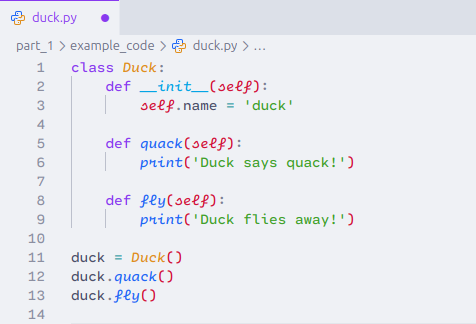
\includegraphics[width=1.0\textwidth]{img/duck_code}
    \end{column}%
  \end{columns}

\end{frame}

\begin{frame}{Très adaptable}
  \begin{columns}[T]
    \begin{column}{.4\textwidth}
      \begin{block}{}
        \begin{itemize}
          \item<+-> Exécution intéractive ou par script
          \item<+-> Multiplateforme et open source
          \item<+-> Correction de bugs \textbf{relativement simple}
        \end{itemize}
      \end{block}
    \end{column}%
    \hfill
    \begin{column}{.6\textwidth}
      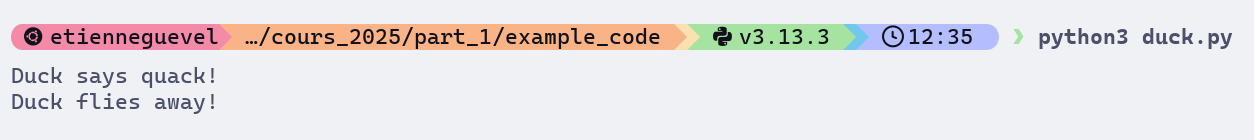
\includegraphics[width=0.85\textwidth]{img/duck_terminal}\\[1ex]
      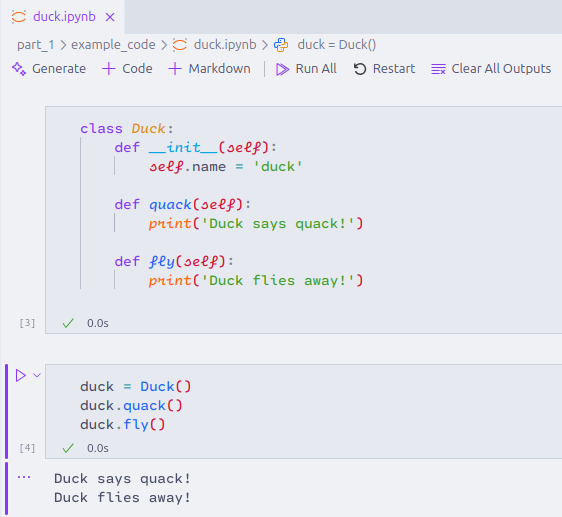
\includegraphics[width=0.85\textwidth]{img/duck_jupyter}
    \end{column}%
  \end{columns}

\end{frame}



\begin{frame}{Mais relativement peu performant}

  \begin{columns}[T]
    \begin{column}{.6\textwidth}
      \begin{block}{}
        \begin{itemize}
          \item<+-> Interprétation vs compilation
          \item<+-> Gestion de données et bibliothèques de haut niveau
          \item<+-> Typage dynamique
          \item<+-> Gestion automatique de mémoire
        \end{itemize}
      \end{block}
    \end{column}%
    \hfill
    \begin{column}{.4\textwidth}
      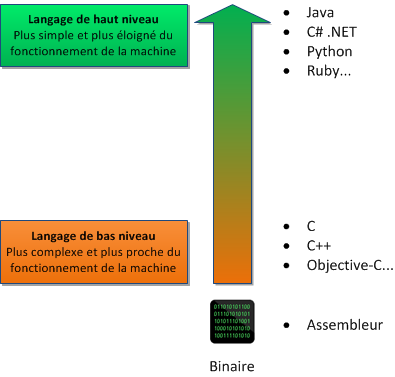
\includegraphics[width=0.85\textwidth]{img/abstraction}
    \end{column}%
  \end{columns}

\end{frame}







\begin{frame}{Une histoire de versions}
  \centering
  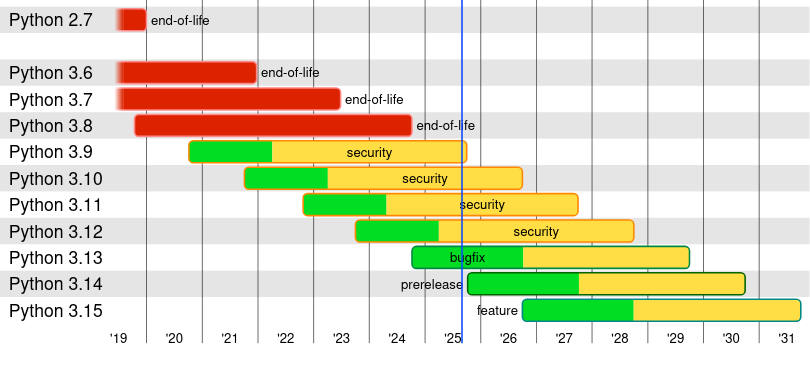
\includegraphics[width=1.\textwidth]{img/python-versions.png}
\end{frame}



\section{Installation et revue des outils}




\begin{frame}{Pré-requis pour le cours}
  \begin{itemize}[<+->]
    \item Un terminal
      \begin{itemize}
        \item Linux / MacOS : le terminal par défaut
        \item Windows : Powershell, intégré à Anaconda
        \item Windows 10 ou 11 (conseil) : Windows Subsystem for Linux
        (\underline{\href{https://learn.microsoft.com/fr-fr/windows/wsl/install}{wsl}})
        
      \end{itemize}
    \item Python, Anaconda, Miniconda version $\geq$ 3.10
    \item jupyter-lab ou jupyter-notebook
    \item Un IDE (ex. VSCode, PyCharm)
  \end{itemize}


\end{frame}



\begin{frame}{Commandes Linux à connaître}
  \begin{center}
    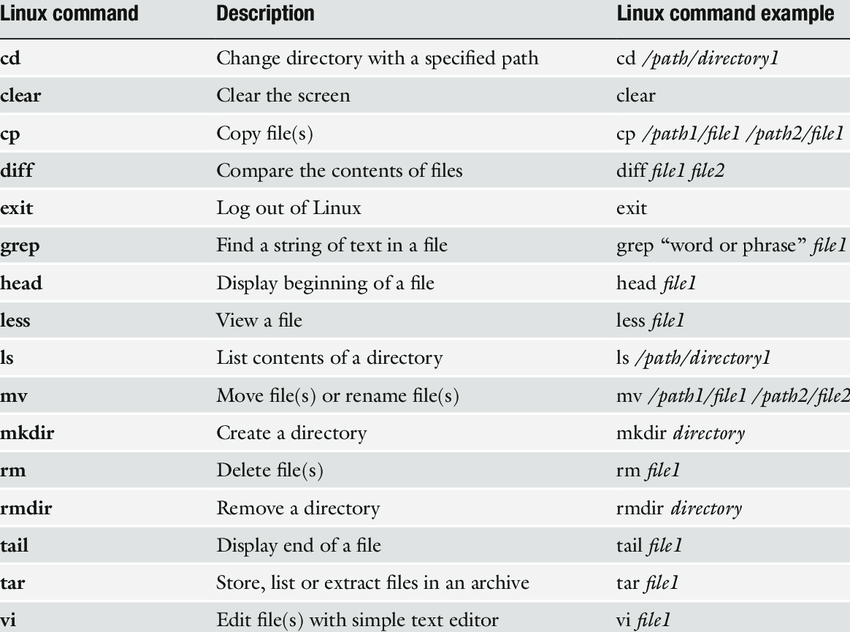
\includegraphics[width=\textwidth]{img/List-of-basic-Linux-commands.png}
  \end{center}
\end{frame}



\begin{frame}[fragile]{Installation de Python}
  Python3 est en général déjà installé, sous Linux 
  \textbf{Python2 est systématiquement installé}.
  
  Il existe plusieurs façons d'installer python (et ses outils) :

\begin{overprint}
  \onslide<1>
    \begin{block}{1/ Paquets Python}
    \medskip
  Pour Linux (ou wsl) :
\begin{lstlisting}[language=bash, morekeywords=\$, numbers=none]
$ sudo apt-get install python3 python3-pip
\end{lstlisting}
  Pour MacOS :
\begin{lstlisting}[language=bash, morekeywords=\$, numbers=none]
$ brew install python
\end{lstlisting}
    \end{block}

  \onslide<2>
    \begin{block}{2/ Anaconda}
    \medskip
      \begin{itemize}
        \item Installation complète de l'environnement
        \item Un très grand nombre de librairies pré-installées
        \item anaconda navigator installé
        \item Multiplateforme : Windows, Linux, MacOS
      \end{itemize}
    \end{block}
    Voir : \url{https://docs.anaconda.com/anaconda/install}

  \onslide<3>
    \begin{block}{3/ Miniconda}
      \medskip
      \begin{itemize}
        \item Installation minimale de l'environnement (480 MB contre 4.4GB)
        \item Aucune librairie installée
        \item anaconda navigator non installé
        \item Multiplateforme : Windows, Linux, MacOS
      \end{itemize}
    \end{block}
    Voir : \small\url{https://docs.anaconda.com/miniconda/miniconda-install/}
\end{overprint}
\end{frame}

\begin{frame}[fragile]{Installation de Python}
  Que Choisir ?
  \begin{itemize}
    \item Python officiel : pour avoir un environnement avec plus de contrôle sur les outils installés
    \item Anaconda : pour avoir un environnement clé en main
    \item Miniconda : pour avoir un environnement minimal avec la possibilité de créer des environnements virtuels avec conda
  \end{itemize}
\end{frame}

\begin{frame}[fragile]{Installation de Python}
  Une fois Python installé, ouvrir un terminal et taper
\begin{lstlisting}[language=bash, morekeywords=\$, numbers=none]
$ python --version
$ python3 --version
\end{lstlisting}
\end{frame}


\begin{frame}{Installation de Python via Anaconda}

  \begin{center}
   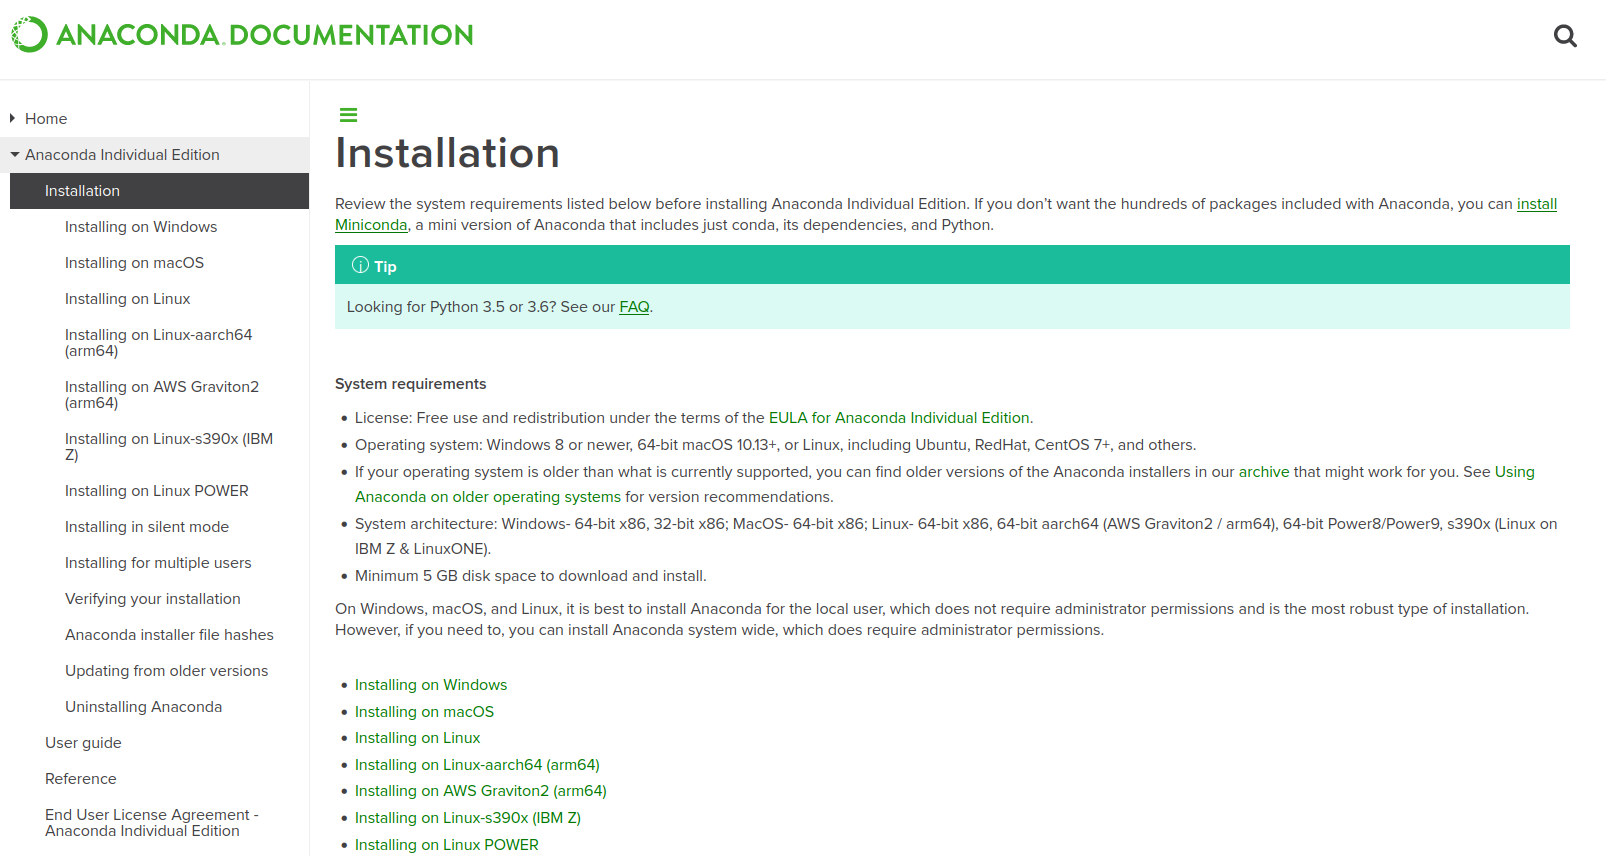
\includegraphics[width=\textwidth]{img/anaconda.png}
  \end{center}
   
\end{frame}
 
 
\begin{frame}{Installation de Python via Anaconda}
  \begin{center}
    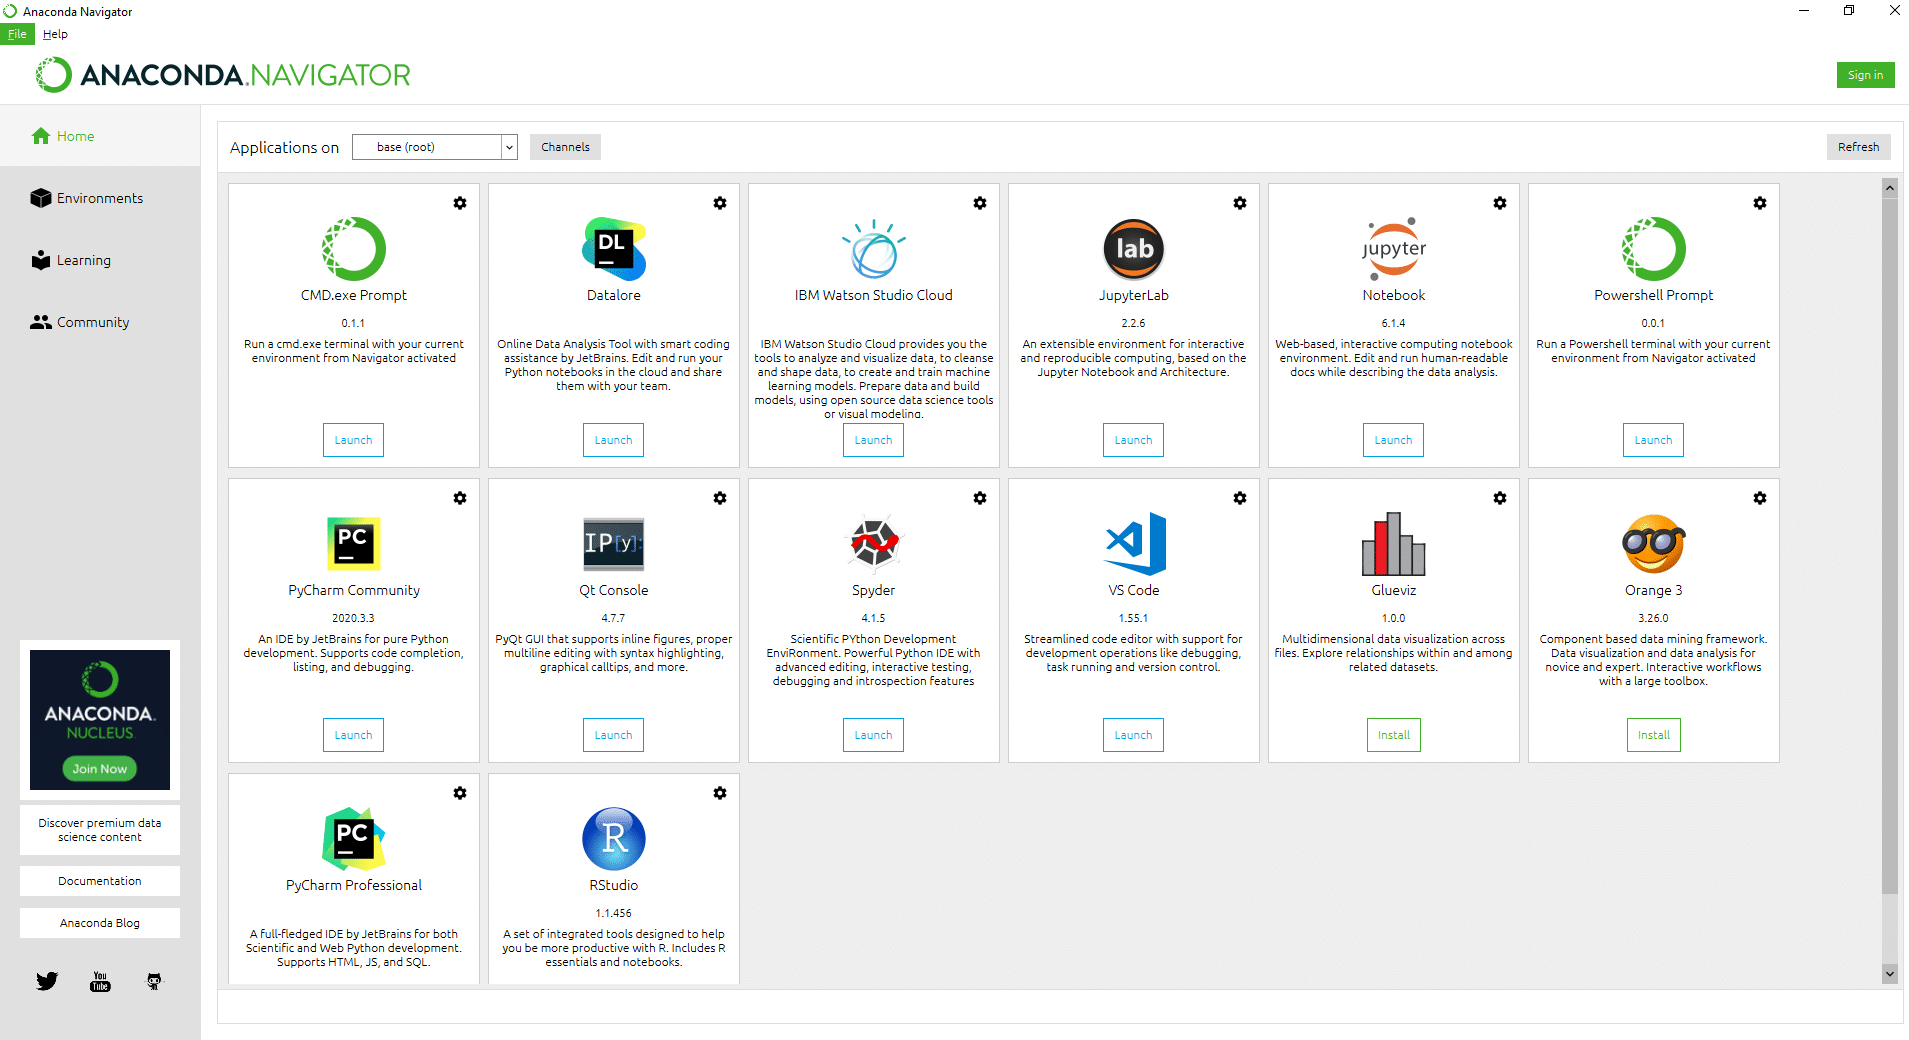
\includegraphics[width=\textwidth]{img/anaconda_navigator.png}
  \end{center}
\end{frame}


\begin{frame}[fragile]{Environnements virtuels}
  Pour gérer des environnements virtuels, avec une installation spécifique
\begin{lstlisting}[language=bash, morekeywords={\$, python, pip, conda, deactivate}, numbers=none]
$ python -m venv myenv
$ source myenv/bin/activate
$ pip install numpy
$ deactivate
\end{lstlisting}
Voir ce
\underline{\href{https://docs.python.org/3/library/venv.html}{lien}}
pour les venvs.

Certaines installations de python viennent sans venv (plutôt pour linux), pour l'installer :

\begin{lstlisting}[language=bash, morekeywords={\$, python, pip, conda, deactivate}, numbers=none]
$ sudo apt install python3-venv # pour linux
\end{lstlisting}
\end{frame}

\begin{frame}[fragile]{Environnements conda}
  Pour gérer des environnements virtuels, avec une installation spécifique
\begin{lstlisting}[language=bash, morekeywords={\$, python, pip, conda}, numbers=none]
$ conda create --name myenv python=3.12
$ conda activate myenv
$ conda install pip
$ pip install numpy
$ conda deactivate
\end{lstlisting}
Voir ce 
\underline{\href{https://conda.io/projects/conda/en/latest/user-guide/tasks/manage-environments.html}{lien}}
pour les envs conda.
\end{frame}

\begin{frame}{Jupyter}
  \begin{center}
    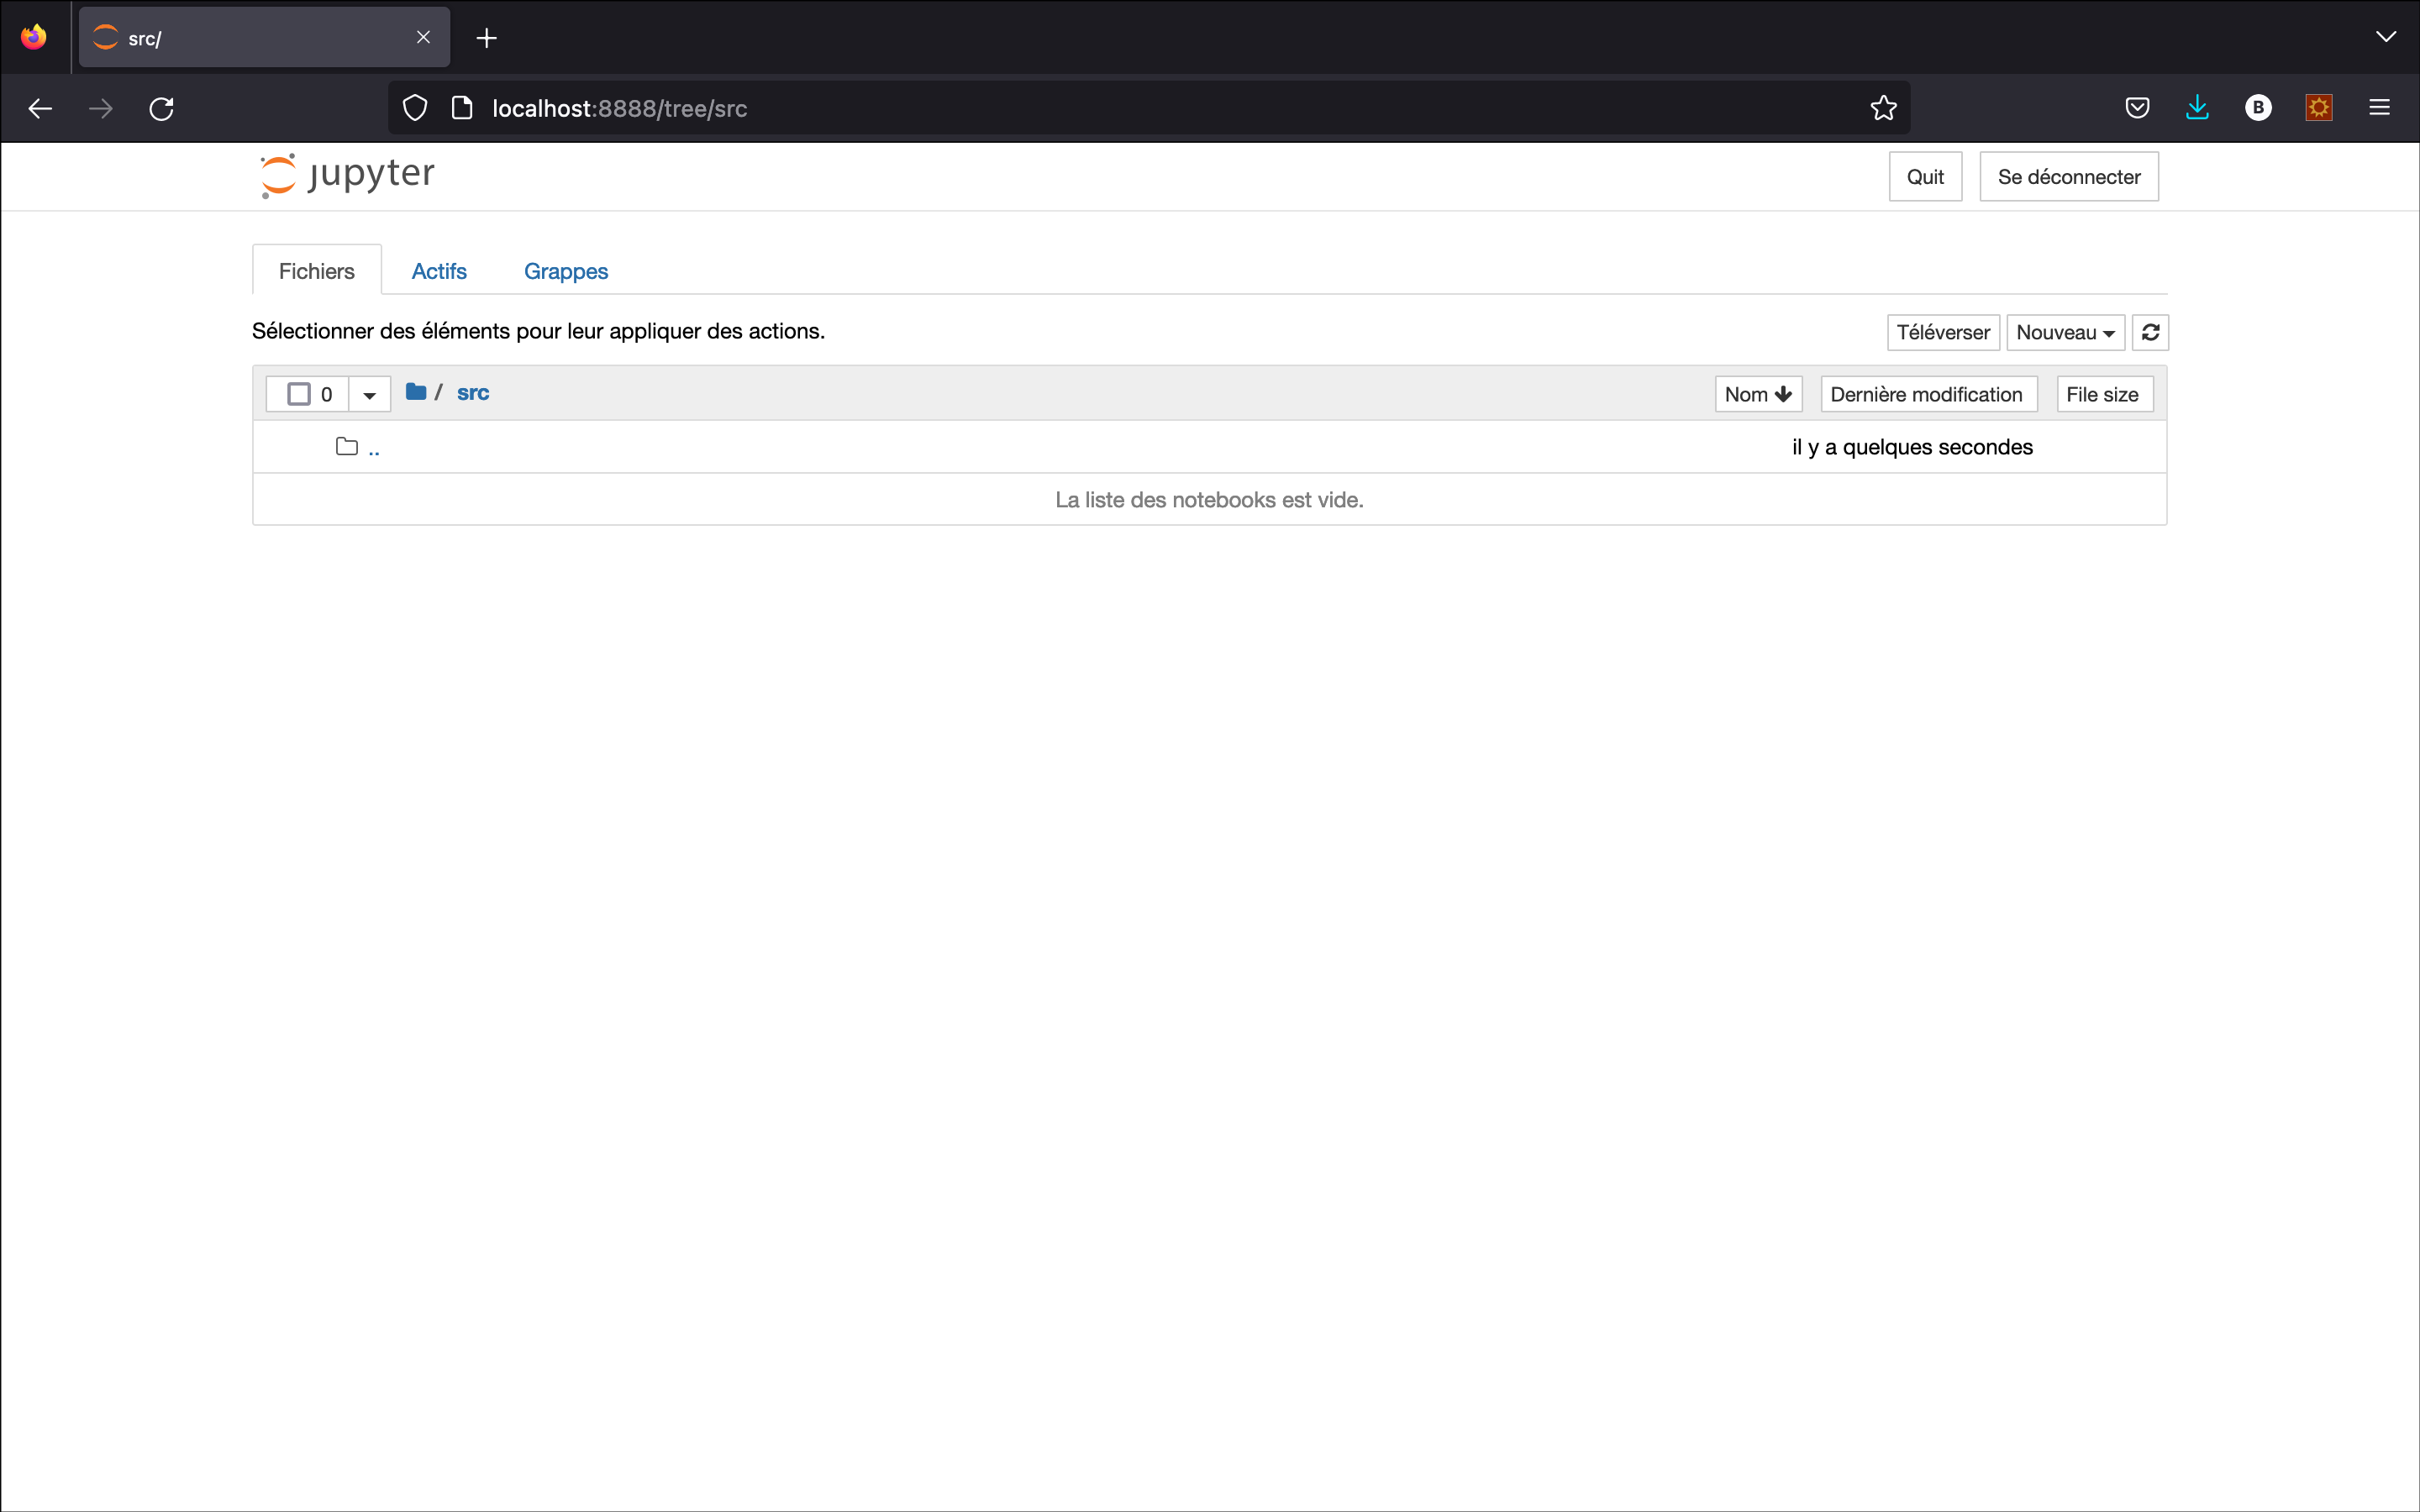
\includegraphics[width=\textwidth]{img/jupyter-nb.png}
  \end{center}
\end{frame}

\begin{frame}[fragile]{Jupyter}
  Pour installer jupyter dans un environnement python via pip :
  \begin{lstlisting}[language=bash, morekeywords=\$, numbers=none]
$ source my_env/bin/activate
$ pip install jupyter # ou notebook ou jupyterlab
$ pip install ipython # package minimal pour vscode notebook
  \end{lstlisting}

    \begin{lstlisting}[language=bash, morekeywords=\$, numbers=none]
$ jupyter lab # ou jupyter notebook
  \end{lstlisting}
  Cela va ensuite ouvrir jupyter dans un navigateur. Si ce n'est pas le cas, un
  lien apparaitra dans le terminal : CTRL + click dessus.
\end{frame}

\begin{frame}{Jupyter}
  \begin{center}
    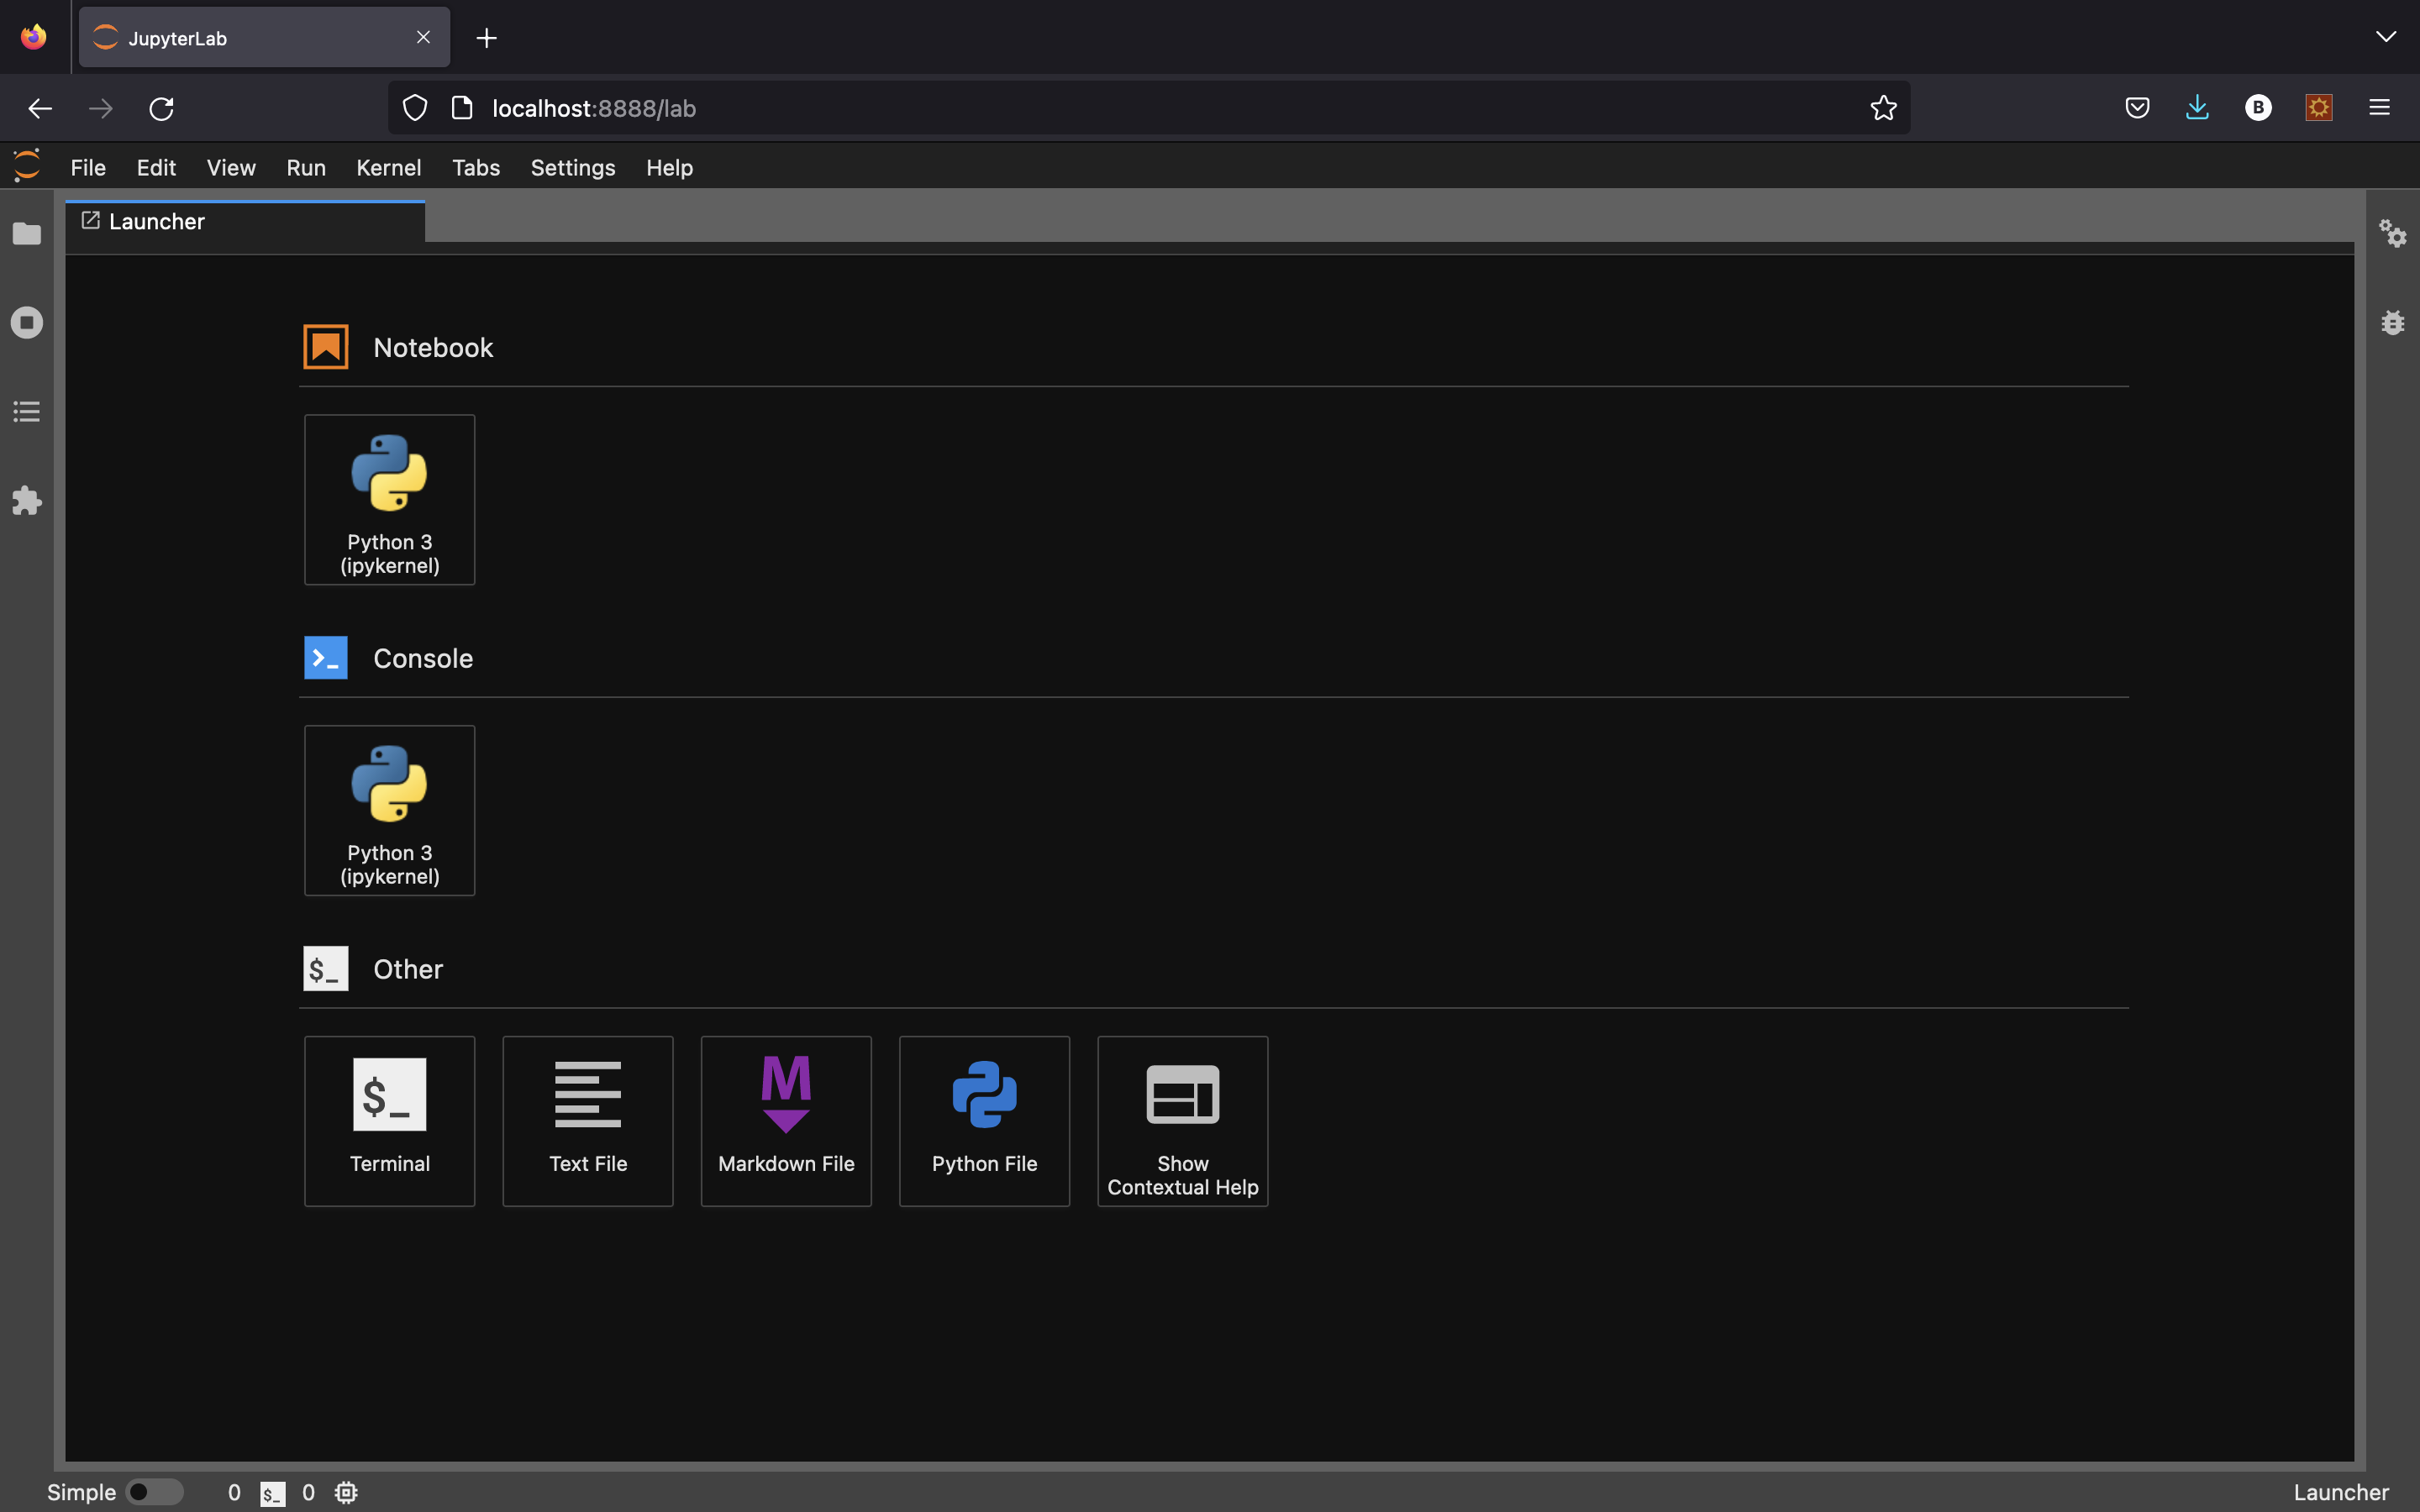
\includegraphics[width=\textwidth]{img/jupyter-lab-1.png}
  \end{center}
\end{frame}

\begin{frame}{Jupyter}
  \begin{center}
    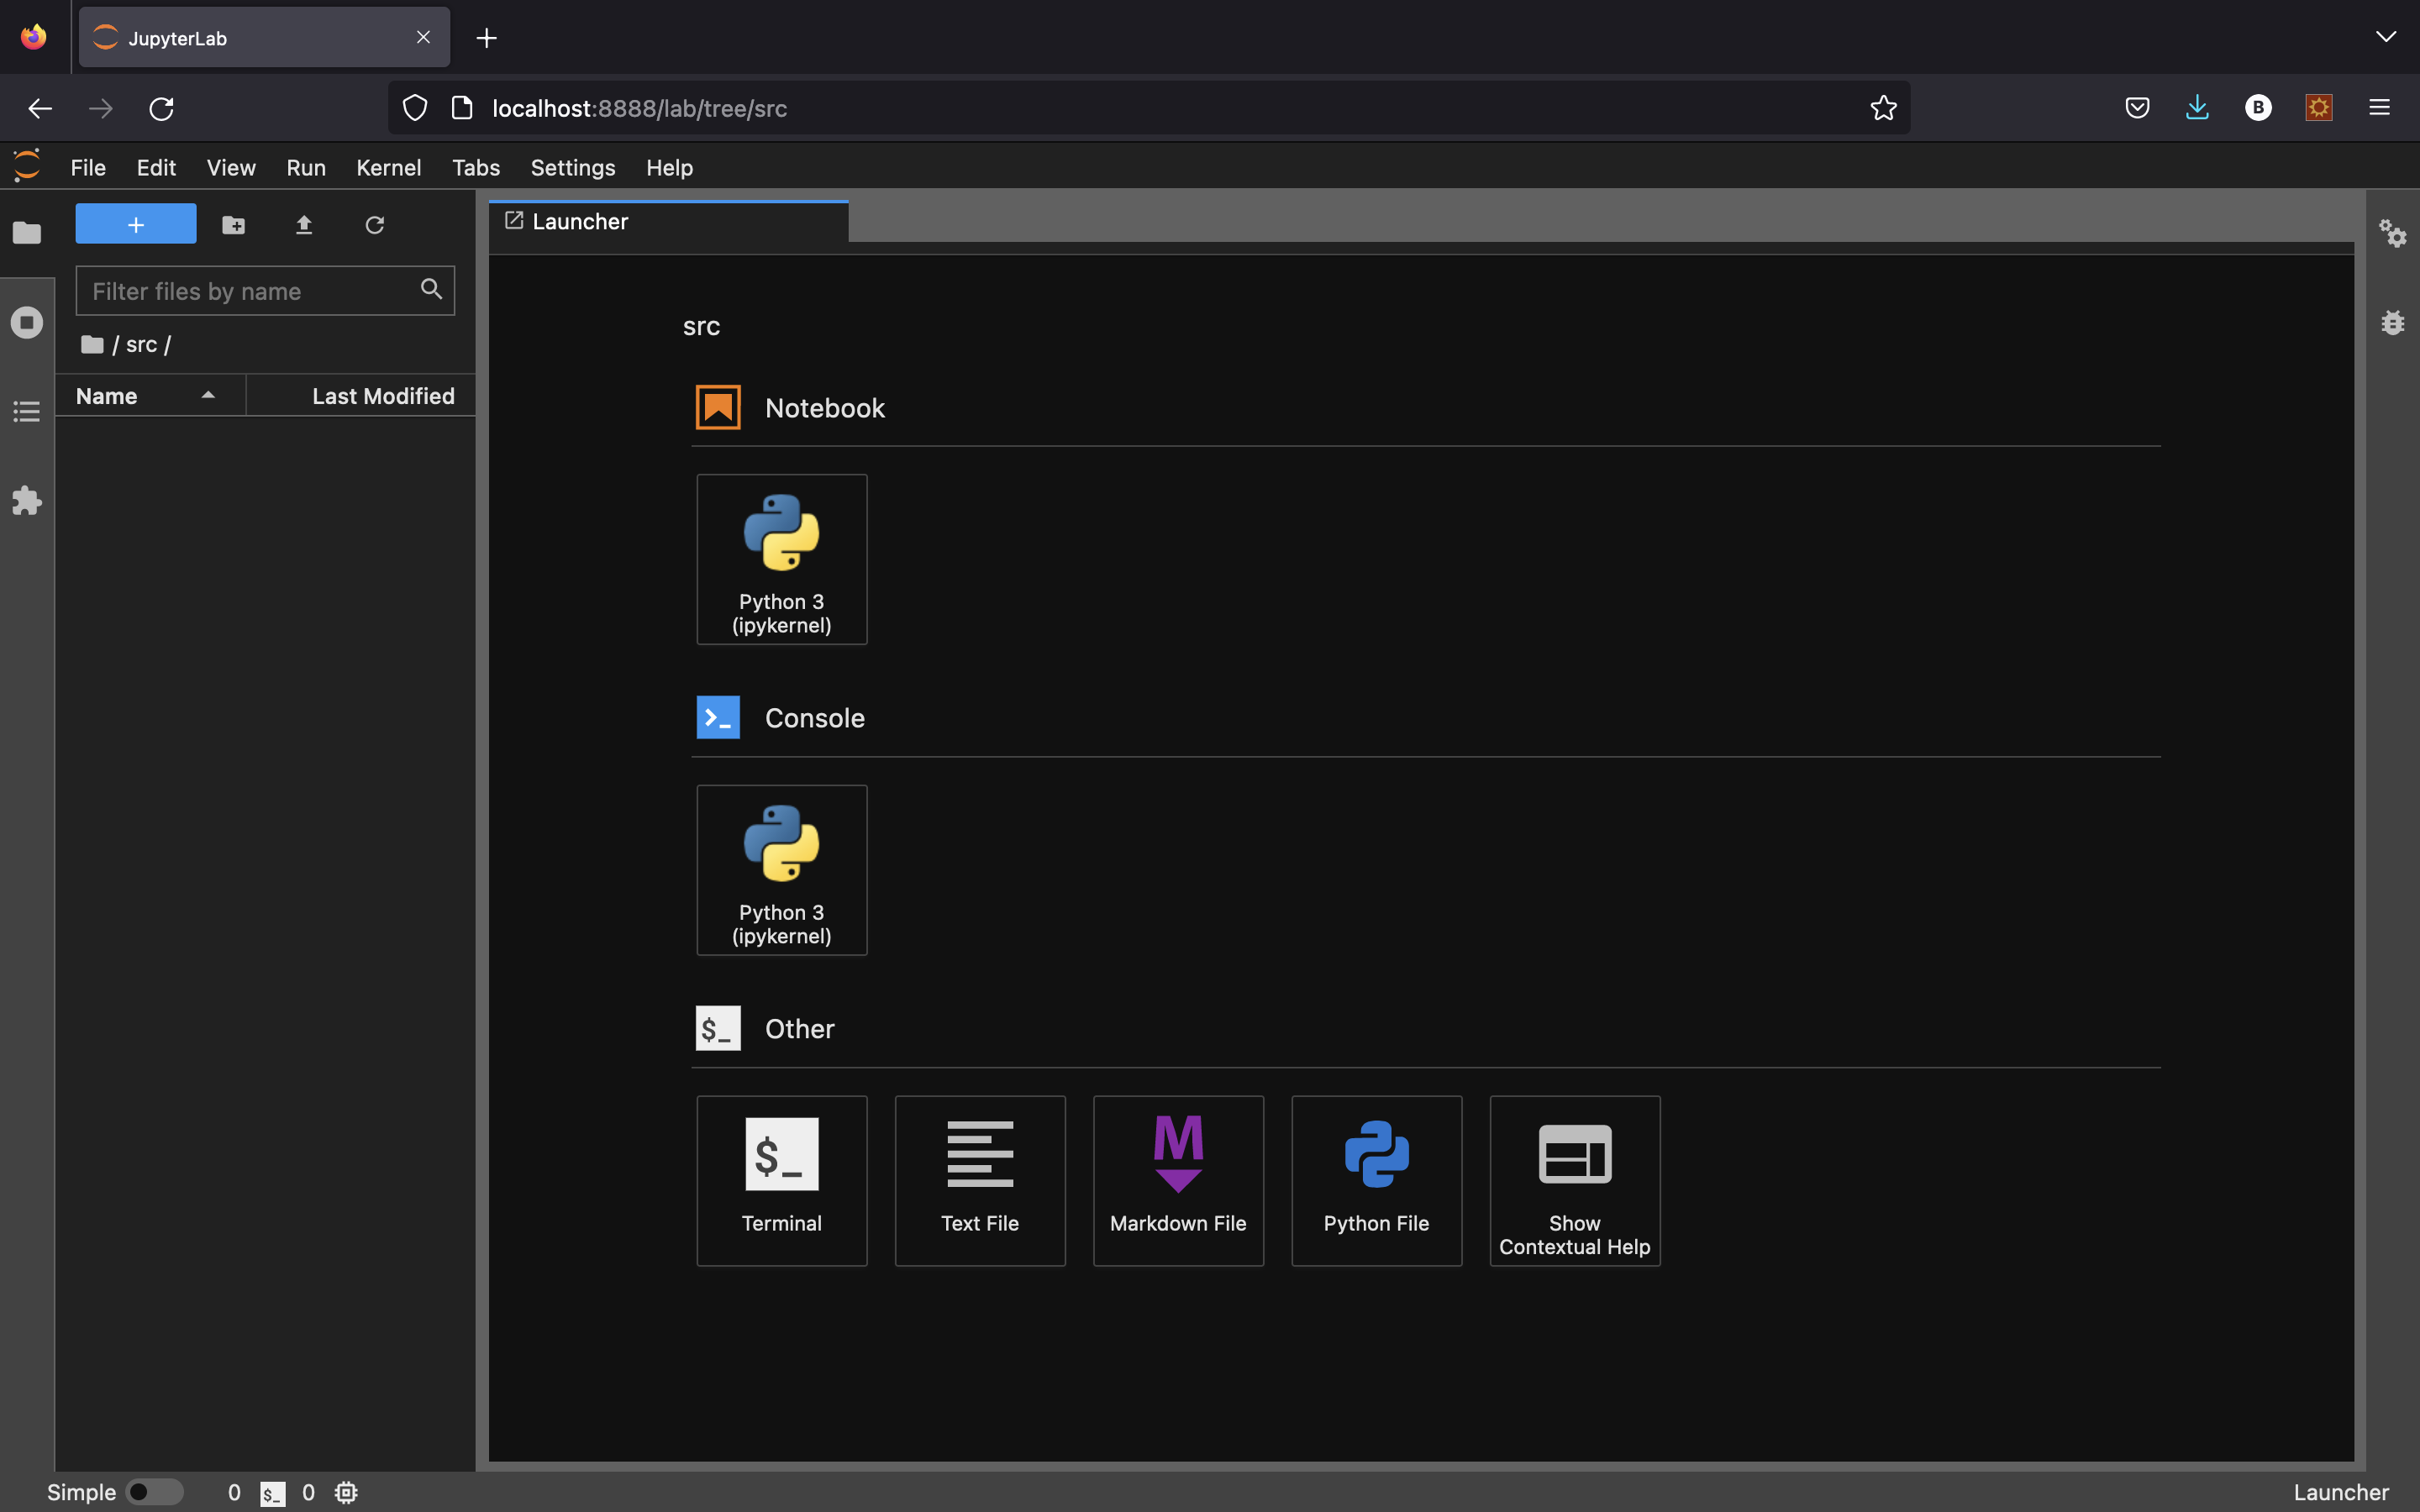
\includegraphics[width=\textwidth]{img/jupyter-lab-2.png}
  \end{center}
\end{frame}

\begin{frame}{Jupyter}
  \begin{center}
    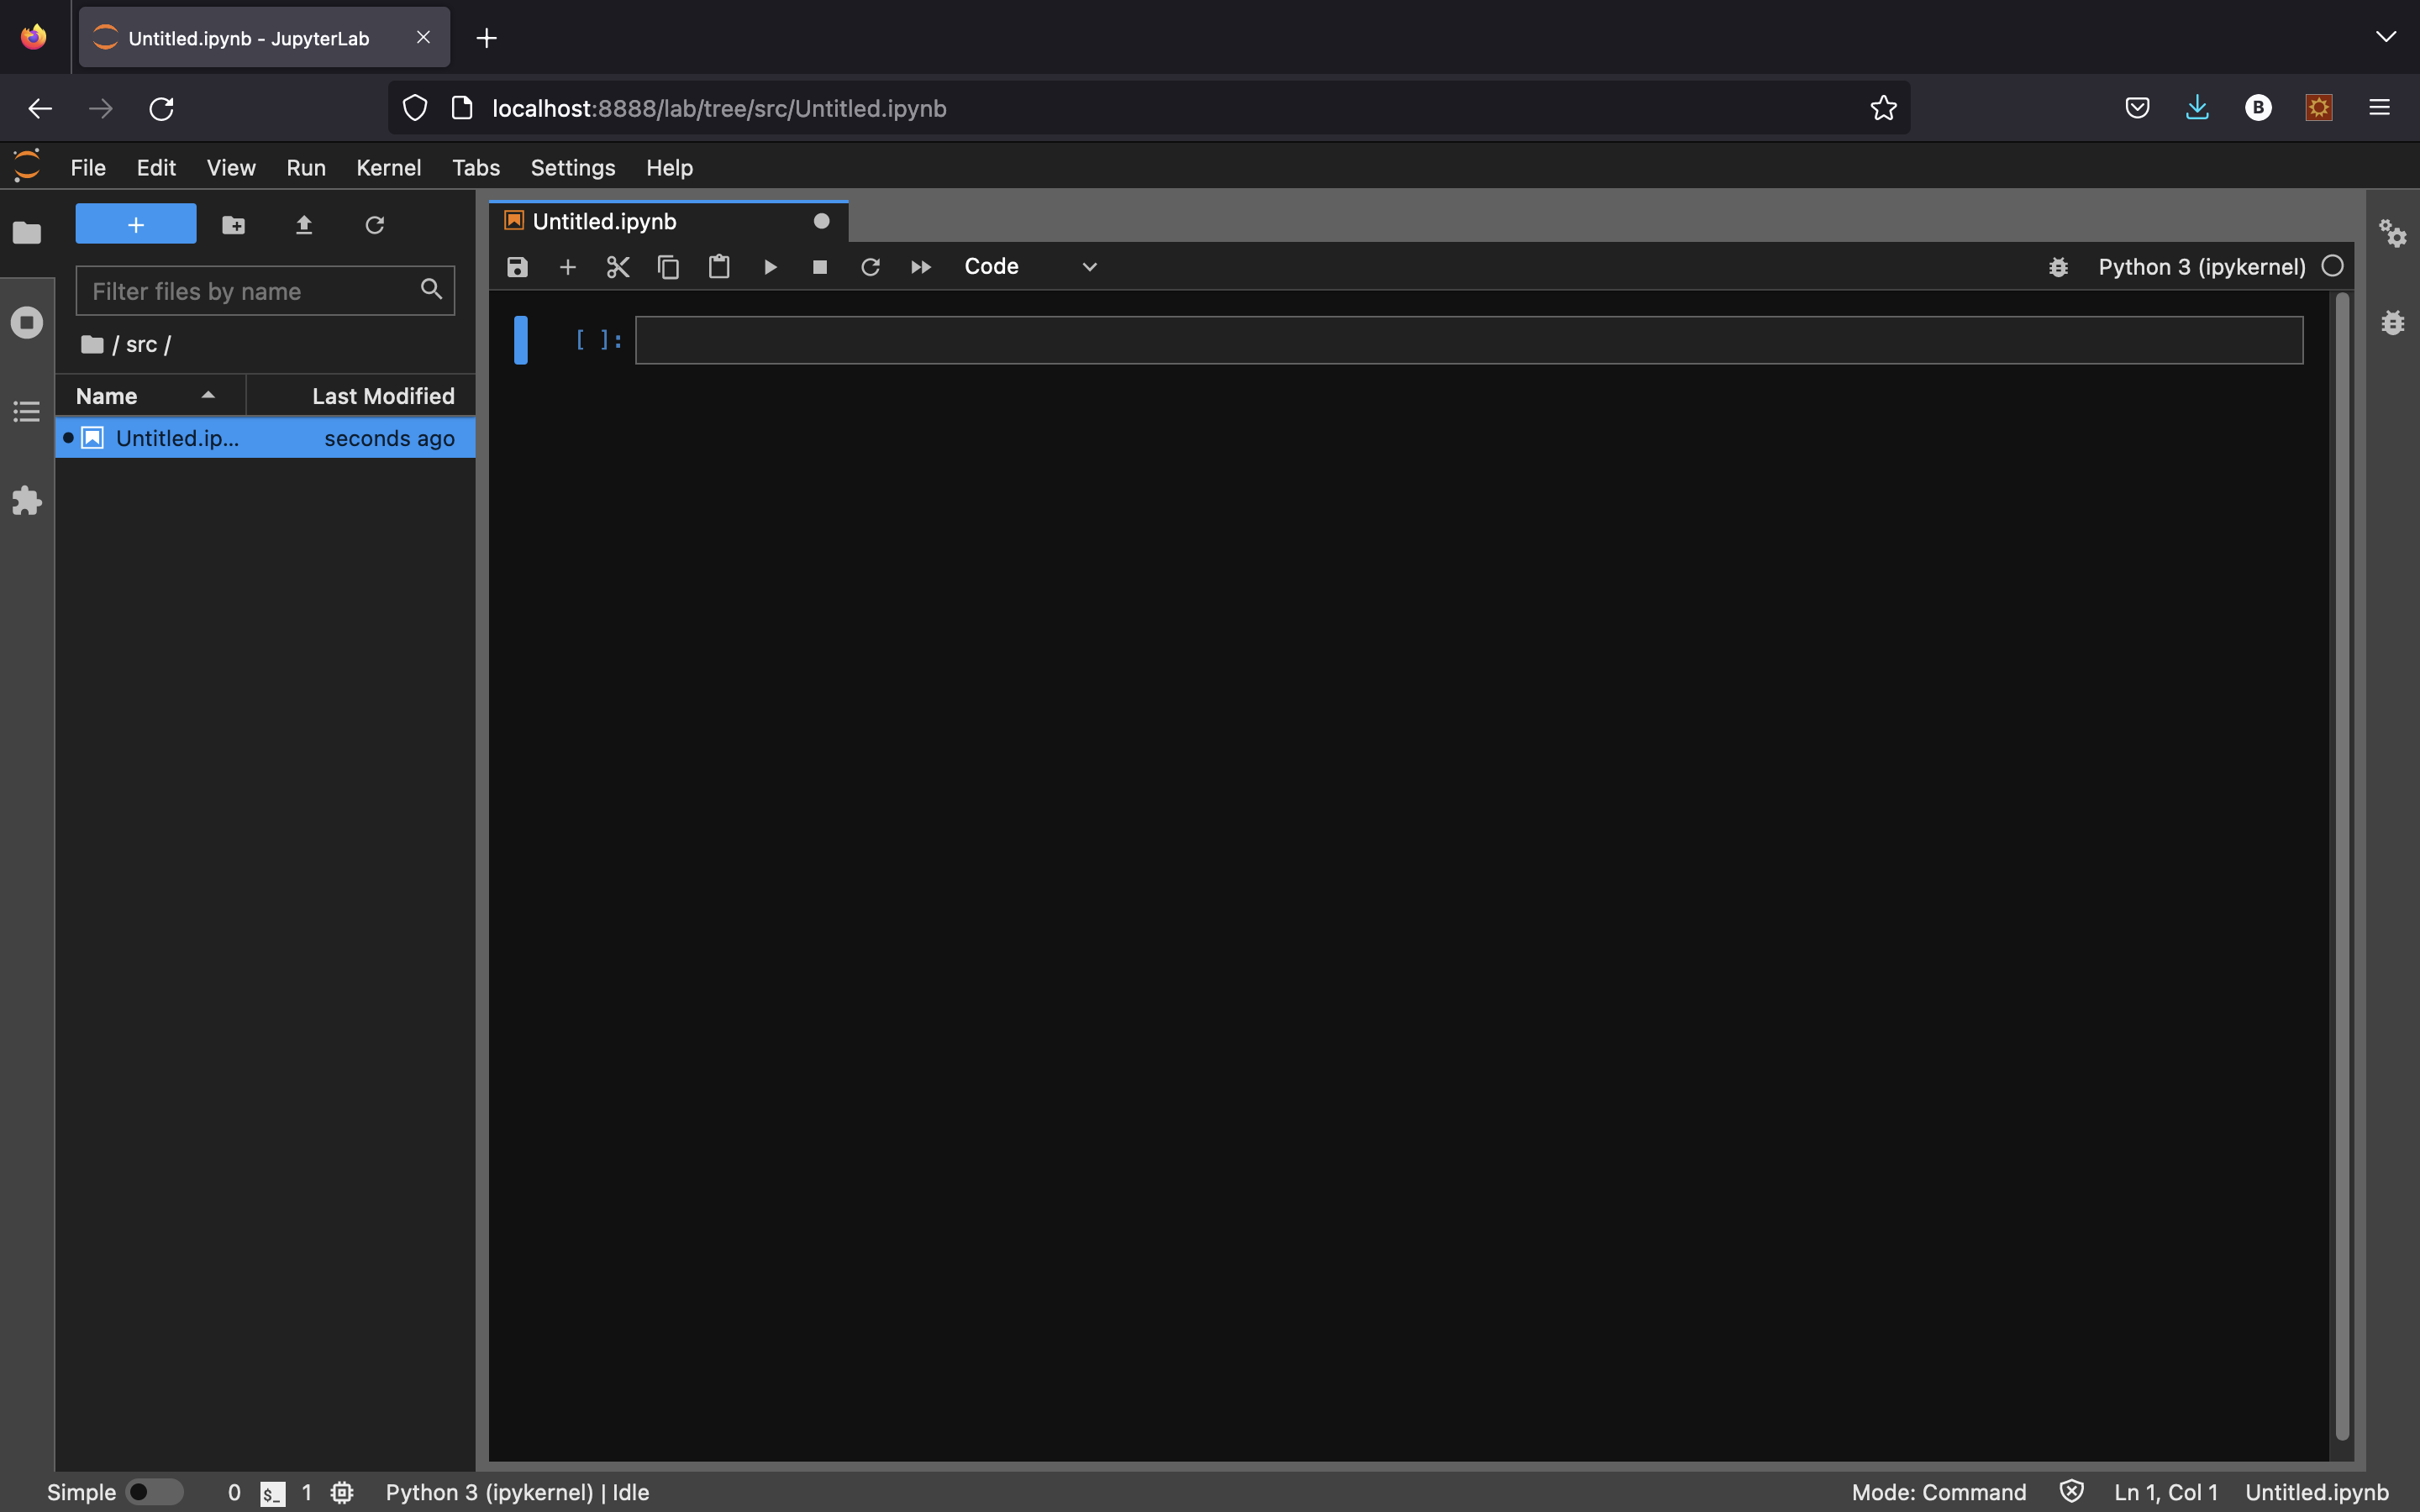
\includegraphics[width=\textwidth]{img/jupyter-lab-3.png}
  \end{center}
\end{frame}


\begin{frame}[fragile]{Exécution d'un programme python}

  \begin{block}{Cas 1 : via un shell python ou ipython}
      \medskip
      Exécution à la volée d'instructions python. Ouvrir un shell
\begin{lstlisting}[language=bash, morekeywords=\$, numbers=none]
$ python
\end{lstlisting}
      Ecrire des instructions
\begin{lstlisting}[language=python, numbers=none]
>>> text = "my name is Etienne Guevel"
>>> print(text)
\end{lstlisting}
  \end{block}

  \begin{center}
    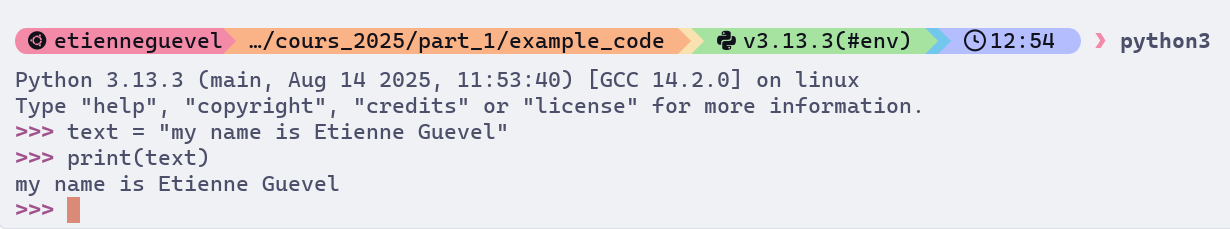
\includegraphics[width=1.\textwidth]{img/print_shell.png}
  \end{center}

\end{frame}
  

\begin{frame}[fragile]{Exécution d'un programme python}

  \begin{block}{Cas 2 : via un terminal}
    \medskip
    Dans un éditeur de texte, créer un fichier \texttt{program.py} et écrire
\begin{lstlisting}[language=python, numbers=none]
text = "my name is Etienne Guevel"
print(text)
\end{lstlisting}

    Exécuter la ligne de commande
\begin{lstlisting}[language=bash, morekeywords=$, numbers=none]
$ python program.py
\end{lstlisting}
  \end{block}

  \begin{center}
    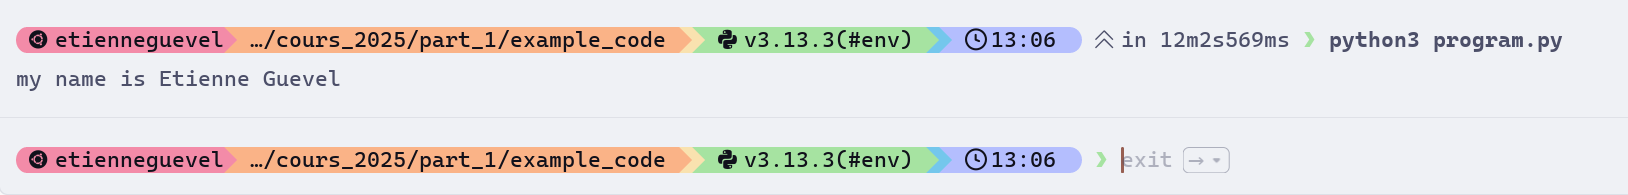
\includegraphics[width=1.\textwidth]{img/dummy_program}
  \end{center}
\end{frame}


\begin{frame}[fragile]{Exécution d'un programme python}

  \begin{block}{Cas 3 : via Jupyter}
    \medskip
    Lancer Jupyter depuis un terminal
\begin{lstlisting}[language=bash, morekeywords=$, numbers=none]
$ jupyter notebook // ou jupyter lab
\end{lstlisting}
    Dans un Jupyter notebook, écrire
\begin{lstlisting}[language=python, numbers=none]
print("Je suis dans Jupyter")
\end{lstlisting}

    et exécuter la cellule correspondante
  \end{block}

  \begin{center}
    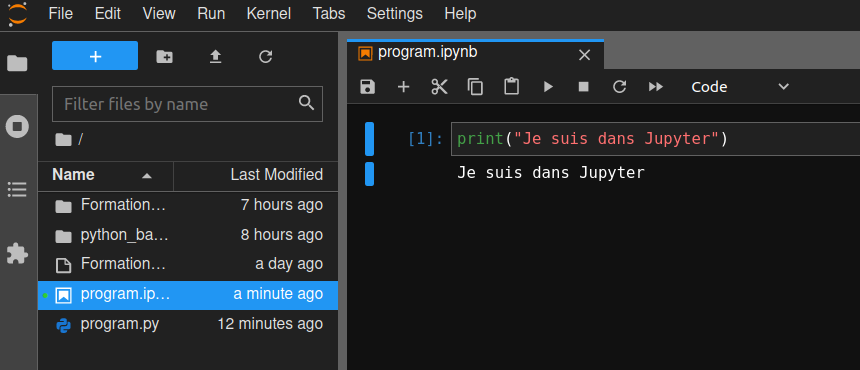
\includegraphics[width=0.7\textwidth]{img/jupyter_program}
  \end{center}
\end{frame}

\begin{frame}{Revue des outils}

  \onslide<1->{
    \begin{block}{Outils de base :}
      \medskip
      \begin{itemize}
        \item python : exécuter du code à la volée
        \item pip : installer des packages
        \item pytest : tests unitaires
        \item pylint : vérification de la qualité du code source
      \end{itemize}
    \end{block}
  }
  \onslide<2>{
    \begin{block}{Intégré au projet Anaconda :}
      \medskip
      \begin{itemize}
        \item ipython : version interactive du shell python
        \item conda : installer des packages, gérer des environnements d'exécutions (voir \href{https://conda.io/projects/conda/en/latest/user-guide/tasks/manage-environments.html}{ici}), etc.
        \item Jupyter : environnement de développement intéractif et fléxible
      \end{itemize}
    \end{block}
  }
  \end{frame}

\begin{frame}[fragile]{Installer des IDEs}
  Les IDEs sont des environnements de développement intégrés (Integrated Development Environment) qui permettent de faciliter la création de programmes.
  \begin{center}
    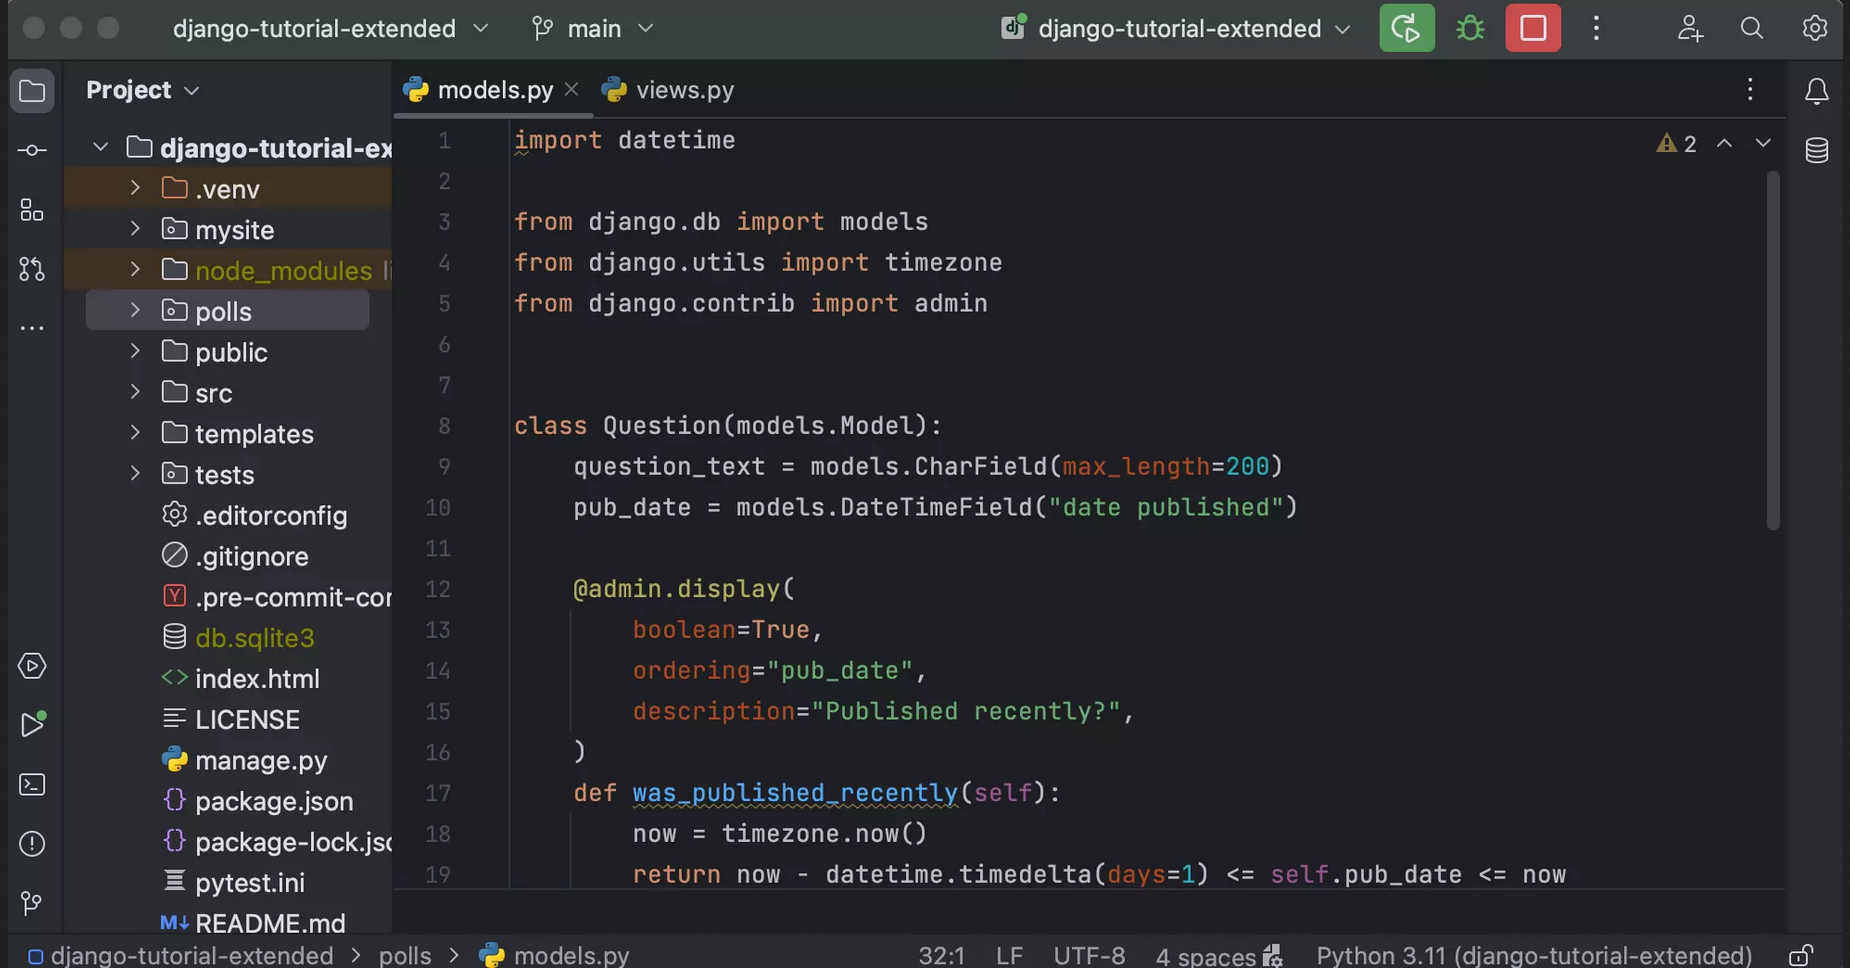
\includegraphics[width=\textwidth]{img/pycharm.png}
  \end{center}
\end{frame}

\begin{frame}[fragile]{Installer des IDEs}
  Les IDEs sont des environnements de développement intégrés (Integrated Development Environment) qui permettent de faciliter la création de programmes.
  \begin{center}
    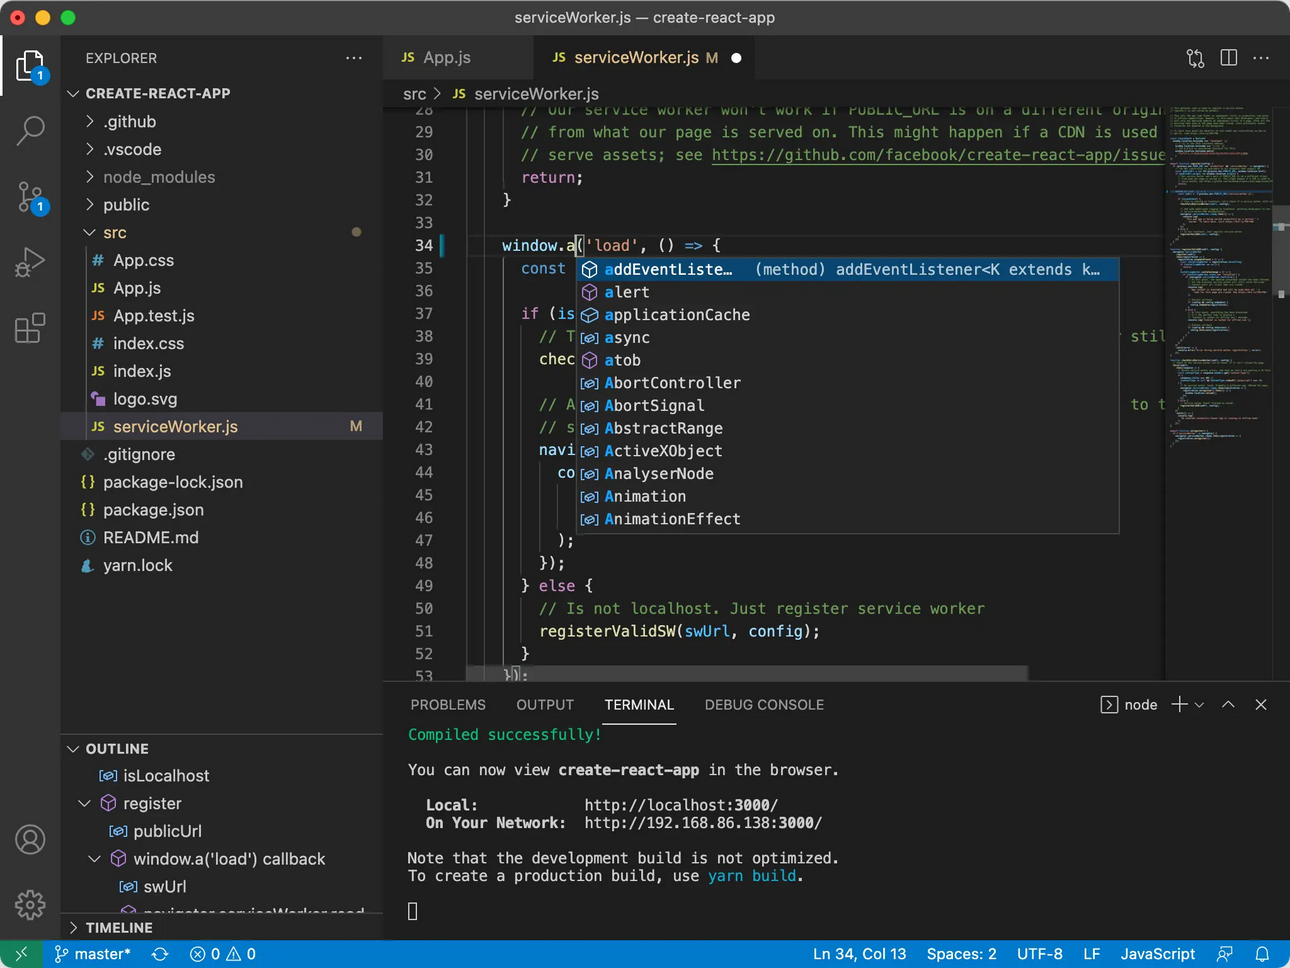
\includegraphics[width=\textwidth]{img/vscode.png}
  \end{center}
\end{frame}

